
\documentclass{IEEEtran}
\IEEEoverridecommandlockouts
% The preceding line is only needed to identify funding in the first footnote. If that is unneeded, please comment it out.
\usepackage{cite}
\usepackage{amsmath,amssymb,amsfonts}
\usepackage{algorithmic}
\usepackage{graphicx}
\usepackage{textcomp}
\usepackage{xcolor}
\def\BibTeX{{\rm B\kern-.05em{\sc i\kern-.025em b}\kern-.08em
    T\kern-.1667em\lower.7ex\hbox{E}\kern-.125emX}}


\begin{document}

\title{Linux security modules and whole-system provenance capture\\
{\footnotesize}
\thanks{}
}

\author{\IEEEauthorblockN{ Aarti Kashyap} \\
\IEEEauthorblockA{\textit{Electrical and Computer Engineering} \\
\textit{ University of British Columbia}\\
Vancouver, Canada \\
kaarti.sr@gmail.com}


}

\maketitle

\section*{Abstract}
	 \textbf{Data provenance describes how data came to be in its present form. It includes data sources and the transformations that have been applied to them. There have been several different OS provenance capture tools in the past. However, only CamFlow and its predecessor Linux Provenance Modules use Linux Security Modules which is a  framework  that allows the Linux kernel to support a variety of computer security models while avoiding favouritism toward any single security implementation. This paper examines the relationship between LSM and CamFlow. the two key research questions that are addressed: 1) Does
	 the latest version of Linux LSM capture all security related information flows? 2) Given the results of #1 and the data captured by CamFlow in its LSM hooks, can we prove that an intrusion will be reflected as a different in the provenance graphs. This is an important question that either validates or refutes the use of kernel provenance for intrusion detection.}








\section{Introduction}
System security is a race between the attackers and the defenders. The attackers adapt their attack model based on the defense mechanisms deployed on systems. The designers of the systems can build a completely correct system using formal methods such as theorem proving and model checking \cite{b4}. However, this only proves the correctness properties of the systems such as " Making sure that the system is following the correct protocol " or  " the shared memory allocation is done efficiently". The attacker can make sure that there is no violation in these properties and still manage to attack the system. In order to beat the attacker in this game, security-based mitigation techniques are proposed, which lack complete security coverage. \cite{b5}. Hence, in order to obtain a full or wider coverage of the system, using provenance-based techniques is an ideal way to proceed. \cite{b6}

Provenance has many different definitions when used in different contexts. The simplest way to define provenance is a formal set of documents, to understand the beginning of something's existence and origin. These documents can be used to guide the authenticity or quality of the item. In a computing context, data provenance represents, in a formal manner, different relationships between entities (data items), activities (data transitions) and agents (which cause the transition). In other words, it can be understood as a formal set of documents which help in understanding the data existence and its flow to trace its integrity (quality). \cite{b1}

Information flow tracking is a security mechanism designed to monitor how sensitive information spreads in a system. In data provenance context, information flow tracking is used to track the data and is be further used to put limits on the dissemination of a piece of sensitive data once it's out of its container of information. This allows high-level policies such as " my banking information will not be sent outside my system " or " my banking information will not be mixed with my wife's banking information" to be enforced easily.  \cite{b2}. Explicit information flow is defined as the copy, usually partial, of the content of one container of information to another. \cite{b3}

Data provenance with a completeness property ensures that all the information flows of the data within the system are being recorded. Pasquier et. al \cite{b6} in his work on Run-time Analysis of Whole-system provenance ensures the completeness and accuracy of the provenance capture mechanism. He further makes use of Georget et al's \cite{b3} formalism to show that all the information flows between the kernel objects are properly recorded. However, this does not prove that all the security-related flows are also being captured by the system. This also does not tell us if the completeness of the information-flow property suffices to find intrusions.


\begin{figure}
	\centering
	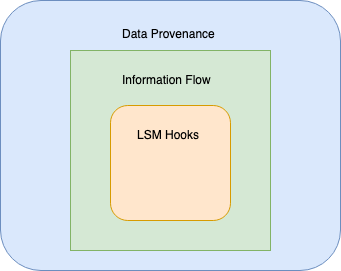
\includegraphics[width=0.7\linewidth]{Architecture-diagram}
	\caption[]{High-level Architectural view. A structured way to formalize whole-system data provenance is to formalize if all the information flows are being captured. In order to make sure that all information flows are being captured we need to make use of LSM to insert hooks at every point in the kernel where a user-level system call is about to result in access to an important internal kernel object.}
	\label{fig:architecture-diagram}
\end{figure}







Hence, as a part of this work we try to answer the question about complete and security-related information flows of the system using a whole-system provenance capture called Camflow.\cite{b7}

The first part of the challenge includes answering the question if the completeness formalism is enough to detect all security related flows. Xueyuan et al. use a whole-system provenance capture tool for fault-detection \cite{b8}. Pasquier et. al. \cite{b6} shows that it's possible to detect intrusions during run-time of the system using CamFlow. However, is it enough to detect all sorts of data leaks and/or intrusions is one question we try to answer as a part of this work? This analysis has been performed for Linux Kernel 4.3. We try to see if the formalism still holds for the updated kernel version (5.0.x).

The second contribution of our work is if indeed Camflow \cite{b7}  is able to capture all security-related flows, do they all show up as an anomaly in the provenance-graph. The provenance-graph is constructed from the data captured from all the security-related flows in the system. 


\begin{figure}
	\centering
	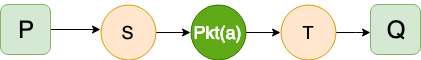
\includegraphics[width=0.7\linewidth]{DAG}
	\caption{A simple provenance DAG: a process P sends packet Pkt(a) to process Q using the sockets S and T.}
	\label{fig:dag}
\end{figure}

\section{Background}
We conduct an analysis to see if the current version of the information flow patch applied to CamFlow is capable enough to catch all security violations. In order to do so, we make use of three open-source tools/libraries/patches CamFlow, GraphChi and complete flow capture formalism proposed by Georget et al \cite{b3}. 

\subsection{CamFlow} 

As we have discussed before data provenance records the chronology of ownership, change, and movement of an object or a resource. There are many provenance capture systems built before CamFlow such as PASS \cite{b10}, Hi-Fi\cite{b11} and Linux Provenance Module (LPM) \cite{b12}. However, none of the above mentioned Operating systems provenance capture systems utilize LSM except for it's predecessor LPM. LSM is a framework that allows the kernel to support a variety of computer security models while avoiding favoritism towards any of the security implementations. 

We chose CamFlow for testing our hypothesis because it adopts the LSM architecture and support for NetFilters which makes it a maintainable practical whole-system provenance implementation.CamFlow maintains an information-flow patch based on Georget et al's \cite{b3}formalism which provides completeness guarantees. The fact that Cam-flow provides completeness guarantees, its a strong choice for researchers to use it as a fault-detection tool \cite{b8}. Pasquier et al. use CamFlow to perform a run-time analysis of whole-system provenance to find intrusions \cite{b6}. However, since the completeness guarantees are specific to kernel version 4.3, we want to provide a formalism which shows that it holds for the updated kernel versions.  

In order to perform such an analysis,  Pasquier et al. have maintained a systematic build script for CamFlow Linux provenance.  This script generates kernel patch for CamFlow Linux provenance capture. It consists of two parts which are running the automated Travis script and  CircleCI script.  The Travis script 

builds the kernel and eventually builds the kernel patch. The CircleCl script performs kernel analysis.

\subsection{GraphChi}

The representation of the provenance data is in the form of a directed acyclic graph (DAG). Every node in the DAG represents an entity, an activity or an agent. Each directed edge represents an interaction between each node. Fig.2 represents a simple example. In our context, entities are kernel objects, activities are tasks, and agents are users and groups. Fig 2 represents packet being sent from process P to Q from socket S to T. 

We use GraphChi, a vertex-centric graph processing model to generate program models and to generate anomalies. The purpose of utilizing GraphChi is to answer that in case of security violations in the system, are the anomalies reflected in the graphs. This is a tool which we use for ensuring if all anomalies are reflected on the provenance graph after the capture. 


\subsection{Formalism of complete mediation}

Georget et al. \cite{b3} proposed a formalism to verify the property for complete capture of the information flows called \textit{Complete Mediation}. The authors use a compiler-assisted and reproducible static analysis on Linux kernel to verify that the LSM hooks are correctly placed with respect to operations generating information flows. This ensures that LSM-based information flow monitors can properly track all information flows.




\section{Evaluation}

The evaluation of the system is performed in two parts. The first part is where we focus on the completeness and accuracy of the current CamFlow patch with respect to the new kernel version. We also try to find if all the security-related flows are being captured by the LSM-interface. The second half of our evaluation focuses on the anomaly detection aspect. We want to prove ( or disprove ) if all security related flows are being captured by the LSM-interface, then the anomaly must show up in the provenance graph.

\subsection{LSM interface and security-related flows}
Before analysing if all security-related flows are being captured by the interface, we first ensure the sompletness and accuracy of the interface





\subsubsection{Completeness}
We want to ensure that all flows of information between kernel objects are properly recorded. The LSM framework \cite{b14} was originally implemented to support Mandatory Access Control (MAC) schemes but not information flow tracking. Georget et al \cite{b3} through static analysis of the kernel code base demonstrated that LSM framework is applicable to information flow tracking. By adding a small number of hooks it is possible to properly intercept all information flows between kernel objects.

In order to run the analysis we use the scripts written by Pasquier et al \cite{b14} which generates the coverage, hooks, relations, stats and vertices for the system. We can see that some of the hooks such as the ones listed in Table 1 are ignored. The automated CircleCl script performs kernel source code analysis and generates the above mentioned attributes in the docs folder. 




From the analysis we observe that the coverage is not complete. Hence, the attacker can still find ways to attack the system. The coverage for different system calls is different. For eg. we observe that for \_\_x64\_sys\_open system call the coverage is 8 out of 12. This means that out of the 12 hooks which were originally called by this system call, only 8 hooks were implemented. We observe similar coverage for different system calls. 

\subsubsection{Security-related flows}
Based on the coverage we observe a couple of security-related flows which will not be captured by the current provenance capturing mechanism.  If the attack is strictly about extracting information from within an application memory, the effect is not observed. 

\subsection{Anomaly detection}
Now that we are aware that some attacks are caught by the capture mechanism and there are some attacks which are not. We try to observe if all the attacks whose flow is being recorded by the capture mechanism if it is reflected on the graph. 

From our evaluation, we understand that if the flow is being recorded it does get reflected on the graph. This is observed from the coverage analysis which we obtained from running the call graph scripts. However, currently, there is no formalism to prove so. So an important and very relevant contribution to this work would be to provide some form of formalism to show that this happens. Hence, my goal is to show some form of formalism before the final submission.  
\section{Conclusion}

After analyzing the results we observe a couple of things about CamFlow architecture, the formalism proposed by Georget et al. and finally about LSM. 

The reason we performed this analysis was to observe the changes which will be required in the CamFlow code-base to make sure it adheres to the latest versions of the kernel. The other reason we carried out this analysis was how feasible is it to maintain CamFlow with respect to the latest kernel releases. The ultimate goal is to have provenance integrated into the mainline Linux kernel. Thus if we can keep up with the versions, it shows that CamFlow is a fully self-contained Linux kernel module. 

Another observation from the results we can notice a clear completeness-security gap. This tells us that there is a lot more work to be done in order to build intrusion detection systems using provenance capture mechanisms. Provenance capture mechanisms can capture only a subset of the possible attacks.

\section* {Discussion Topics}
The first interesting discussion point is understanding the completeness-security gap if any. Currently, the DAGs are generated with respect to the provenance data. However, this is not taking the timing aspect into consideration. Provenance capture mechanisms currently are data related. The way we can capture anomalies is by learning the data pattern from previous immutable data. However, if the attacker brings in the timing aspect, keeping the data intact can that cause damage? It depends on the application if data delays can cause harm. 

Another interesting point to discuss would be the completeness of information flows means that it guarantees that all flows are being captured. So you need to place hooks at the relevant places which ensures that all information flow paths are being recorded. However, again this does not cover the event aspect of the system. What if instead of modifying the data with alone or modifying the data with respect to time, it modifies the event in a smart way such that the correlations created by the DAG cannot spot it.  Instead of sending the data from process P to process Q, it sends it to process R. 
\section*{Acknowledgment}

This work was done as a part of our term project for CPSC 508. CPSC 508 is a graduate level operating systems course taken by Dr. Margo Seltzer.

\begin{thebibliography}{00}
\bibitem{b1} Lucian Carata, Sherif Akoush, Nikilesh Balakrishnan, Thomas Bytheway,
Ripduman Sohan, Margo Seltzer, Andy Hopper, an ``A Primer on Provenance,'' acmqueue, 2014.
\bibitem{b2} Daniel Crawl and Ilkay Altintas , A Provenance-Based Fault Tolerance Mechanism for
Scientific Workflows.

\bibitem{b3} Laurent Georget, Mathieu Jaume, Guillaume Piolle, ``Verifying the reliability of operating system-level information flow control systems in linux,'' Proceedings of the 5th International FME Workshop on Formal Methods in Software Engineering, FormaliSE ’17, pages 10–16, Piscataway, NJ, USA, 2017. IEEE Press.

\bibitem{b4}GERWIN KLEIN, ``Operating system verification—An overview,"Sadhan ¯ a¯ Vol. 34, Part 1, February 2009, pp. 27–69. © Printed in India

\bibitem{b5} Jonathan Pincus and Brandon Baker , ``Mitigations for Low-Level Coding Vulnerabilities:
Incomparability and Limitations ,'' 2004.


\bibitem{b6}Thomas Pasquier, Xueyuan Han, Thomas Moyer, Adam Bates, Olivier Hermant, David Eyers, Jean Bacon, Margo Seltzer, ``Runtime Analysis of Whole-System Provenance
,''16 pages, 12 figures, 25th ACM Conference on Computer and Communications Security 2018.



\bibitem{b7} Thomas Pasquier, Xueyuan Han, Mark Goldstein, Thomas Moyer, David Eyers, Margo Seltzer, Jean Bacon, Practical Whole-System Provenance Capture
, SoCC '17 Proceedings of the 2017 Symposium on Cloud Computing.


\bibitem{b8} Xueyuan Han, Thomas Pasquier, Tanvi Ranjan, Mark Goldstein, and Margo Seltzer, Harvard University

 , ``FRAPpuccino: Fault-detection through Runtime Analysis of Provenance ,'' HotCloud'17.



\bibitem{b9} PASQUIER, T. F.-M., SINGH, J., BACON, J., AND EYERS, D. , ``Information flow audit for paas clouds.
Cloud Engineering
(IC2E), 2016 IEEE International Conference on (2016), IEEE,
pp. 42–51.


\bibitem{b10} MUNISWAMY-REDDY, K.-K., HOLLAND, D. A., BRAUN, U.,
AND SELTZER, M. I. , `` Provenance-aware storage systems. ,'' In
USENIX Annual Technical Conference, General Track (2006),
pp. 43–56..


\bibitem{b11} POHLY, D. J., MCLAUGHLIN, S., MCDANIEL, P., AND BUTLER, K , ``Hi-fi: collecting high-fidelity whole-system provenance ,'' In Proceedings of the 28th Annual Computer Security Applications Conference (2012), ACM, pp. 259–268.


\bibitem{b12} Adam Bates, Dave (Jing) Tian, and Kevin R.B. Butler , ``Trustworthy Whole-System Provenance
for the Linux Kernel.
24th USENIX Security Symposium, 2015.








\bibitem{b13} PASQUIER, T. , ``Camflow information flow patch.
In https://github. com/CamFlow/information- flow- patch.
.


\bibitem{b14} 	Chris Wright,	
Crispin Cowan,	
Stephen Smalley,	
James Morris,	
Greg Kroah-Hartman.	
, ``Linux Security Modules: General Security Support for the Linux Kernel.
Proceeding
Proceedings of the 11th USENIX Security Symposium
Pages 17-31 

August 05 - 09, 2002 .


\bibitem{b15} PASQUIER, T. , ``CamFlow development.
In https://github.com/CamFlow/camflow-dev.

\bibitem{b16} INRIA , ``The Kayrebt Toolset
In http://kayrebt.gforge.inria.fr/
\end{thebibliography}




\end{document}
